\chapter{DCF77}
\section{Inleiding}
In dit onderdeel, genaamd DCF77,  wordt de basis van de wekker gelegd, door verschillende belangrijke datasignalen aan te maken, welke nodig zijn om de rest van de wekker goed te laten functioneren. Een eis die is gesteld aan de eigenschappen van deze klok, is dat deze gesynchroniseerd wordt met het zogenaamde DCF77 signaal. Dit is een signaal dat vanuit Duitsland wordt verzonden en bestaat uit korte (100 ms) en lange (200 ms) pulsen, welke respectievelijk nullen en enen coderen. Iedere seconde, behalve de laatste van iedere minuut, wordt er een puls verzonden. De bits die door deze pulsen worden gecodeerd, bevatten allerlei informatie, zoals de actuele datum en tijd op de eerstvolgende minuut. Een deel van de informatie die op deze manier wordt verzonden, zal worden gebruikt voor het aansturen van de wekker. Om gebruik te kunnen maken van de informatie die met het DCF77 signaal wordt verzonden, is het echter wel nodig te weten welke bit uit de reeks van 59 stuks welke informatie codeert. In figuur \ref{fig:dcfsignaal} is te zien welke informatie door elk van de 59 bits wordt gecodeerd. Een versie in tabelvorm is te vinden op Wikipedia ~\cite{Tijdwiki}. De wekker zal gebruik gaan maken van bits 21 t/m 58. In de afbeelding worden binnen deze selectie bits 28, 35 en 58 respectievelijk P1, P2 en P3 genoemd. Deze bits zijn zogenaamde parity-bits, welke de ontvanger van het DCF77 signaal in staat stelt om tot op zekere hoogte te controleren of de ontvangen bitreeks correct is. In het DCF77 signaal wordt gebruik gemaakt van even parity. Dit betekent dat, wanneer zich in de bits die bij een zekere parity bit horen een even aantal logische enen bevindt, de parity bit een logische 0 zal zijn ~\cite{Tijdscodering}. Het DCF77 blok converteert een gedigitaliseerde versie van het DCF77 signaal naar een tijdreferentie, waarna deze een autonome klok synchroniseert, welke zich ook binnen het DCF77 blok bevindt.

\begin{figure}[h!]
\center
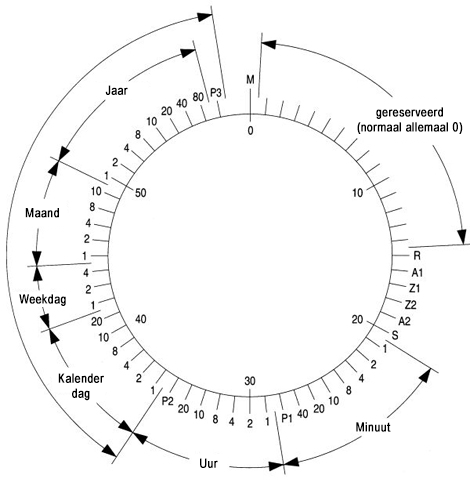
\includegraphics[scale=1.9]{Figuren/DCF77/dcf77coding.png}
\caption{Codering van het dcf-signaal~\cite{Tijdscodering}}
\label{fig:dcfsignaal}
\end{figure}

\section{Specificaties}
In deze sectie worden de in- en uitgangen van de DCF-controller overzichtelijk weergeven. Doordat dit onderdeel aan het begin staat van het totale systeem, bevat dit blok enkel standaard ingangen en een ingang van buitenaf met het DCF77 signaal. De uitgangen uren en minuten worden doorgestuurd naar de main-controller. De clk van 1 Hz zal in verschillende onderdelen worden gebruikt, zowel binnen als buiten het DCF77 blok. De datum en het signaal dcf\_led zullen rechtstreeks op het LCD scherm worden weergegeven. Enkele signalen zijn in BCD (Binairy Coded Decimal). Meer informatie over BCD is te vinden op de website van Technology UK ~\cite{BCDinfo}.

\subsection{Ingangen}
Dit onderdeel maakt gebruik van de volgende ingangen: 
\begin{itemize}[nolistsep]
\item De 32 kHz systeemklok, een standaard input.
\item Het 'active high' resetsignaal, een standaard input.
\item Het gedigitaliseerde DCF77 signaal, bestaande uit korte en lange pulsen.
\end{itemize}
\noindent

\subsection{Uitgangen}
Dit onderdeel genereert de volgende uitgangen:
\begin{itemize}[nolistsep]
\item Een kloksignaal met een frequentie van 1 Hz, welke gebruikt kan worden om secondes te tellen.
\item Het debug signaal dcf\_led, wat een seconde lang hoog is na ontvangst van een puls van het DCF77 signaal.
\item Uren; de uren van de huidige tijd in een BCD vector van 6 bits.
\item Minuten; de minuten van de huidige tijd in een BCD vector van 7 bits.
\item Weekdag; de dag van de week, binair gecodeerd met maandag als 001.
\item Dag; de dag van de maand in een BCD vector van 6 bits.
\item Maand; het nummer van de maand in een BCD vector van 5 bits.
\item Jaar; de laatste twee cijfers van het jaartal in een BCD vector van 8 bits.
\item Date\_ready; een signaal dat aangeeft dat de datum gereed is voor verder gebruik.
\end{itemize}

\subsection{Gedrag}
Het DCF77 blok heeft als belangrijkste gedragsfunctie om de huidige tijd en datum door te geven. Om deze informatie zo precies mogelijk te houden, dient deze zo vaak mogelijk te worden gesynchroniseerd met het extern gedigitaliseerde DCF77 ingangssignaal. Idealiter zou er dus iedere minuut met het DCF77 signaal worden gesynchroniseerd. Pas als via de parity bits is gebleken dat het de ontvangen tijd en datum plausibel zijn, wordt dit echter gedaan. Anders blijft de datum onveranderd en wordt de tijd bijgehouden met een interne klok. Zo wordt voorkomen dat andere onderdelen op de chip tijdelijk een compleet verkeerd signaal krijgen doorgestuurd, indien het DCF-signaal signaal niet of slecht wordt ontvangen.\\

\noindent Naast deze belangrijkste functie, heeft het DCF77 blok ook nog enige kleinere taken. Zo dient het 1 Hz signaal dat afkomstig is uit een interne klokdeler en wordt gebruikt voor de interne klok ook beschikbaar te worden gesteld voor gebruik in andere blokken. Ook dient een debug signaal dcf\_led gegenereerd te worden, dat na iedere ontvangen bit uit het DCF77 signaal een seconde lang hoog is. Ten slotte dienen alle subblokken, inclusief registers, van de gehele module bij een 'active high' reset gereset te worden.

\section{Functionaliteit}
Het DCF blok dient volgens de specificaties een tijd- en dagstempel te genereren uit het gedigitaliseerde DCF77 signaal dat aan het blok wordt aangeboden. Bovendien dient het blok de tijd zelf bij te houden wanneer het DCF77 signaal niet of niet goed wordt ontvangen. Het is vrij ondoenlijk om deze volledige functionaliteit in \'e\'en keer te implementeren in VHDL. Bovendien zou dit een groot, lomp blok opleveren in de layout, welke vervolgens lastig op de chip te plaatsen zal zijn. Daarom wordt het DCF blok opgedeeld in kleinere subblokken, totdat deze wel in \'e\'en keer geïmplementeerd kunnen worden. Een top-level beschrijving knoopt vervolgens de kleinere subblokken weer aan elkaar tot een groot blok. Naast het voordeel dat dit het ontwerpen vergemakkelijkt, geeft dit ook een gemakkelijker op de chip te plaatsen ontwerp, omdat ook de layout op dezelfde hi\"erarchische manier gegenereerd zal worden. \newpage

\noindent In \cref{fig: dcf_subblokken} is te zien hoe het DCF blok is verdeeld in subblokken. Het DCF77 signaal wordt allereerst aangeboden aan het subblok edge detector, welke dit signaal vervolgens opsplitst in twee afzonderlijke signalen. Het eerste signaal geeft een puls wanneer er een rising edge plaatsvind op het DCF77 signaal en het tweede signaal geeft een puls wanneer er een falling edge plaatsvind op het DCF77 signaal. Beide signalen worden doorgevoerd naar de DCF counter, welke het tijdsverschil tussen de rising en falling edges telt. De tellerwaarde wordt na iedere ontvangen puls beschikbaar gesteld aan de daadwerkelijke DCF decoder door het signaal new\_bit hoog te maken.\\

\noindent De DCF decoder bepaald vervolgens wat de bitreeks is die in \'e\'en minuut van het DCF77 signaal gecodeerd is en genereerd hieruit de signalen voor de tijd en datum. Ook de parity bits worden apart naar buiten gevoerd, zodat deze kunnen worden gebruikt in de parity check. Naast deze signalen genereert de decoder ook het debug signaal dcf\_led, dat aangeeft of het DCF77 signaal goed wordt ontvangen. Ten slotte genereert de decoder een signaal ``start'' dat aangeeft wanneer een volledige minuut is gedecodeerd. Dit laatste signaal gaat, samen met de tijd-, datum- en parity bits naar het subblok parity check. Hier wordt gecontroleerd of het aantal enen (even of oneven) klopt met wat het parity bit aangeeft. Het parity bit is namelijk alleen 0 wanneer er een even aantal bits bij hoort. Het controleren op een even of oneven aantal enen gebeurt door middel van een herhaalde xor operatie. Het subblok parity check genereert vervolgens een sync\_now signaal dat aangeeft dat de controle is voltooid en succesvol was. Dit signaal wordt ook naar buiten gevoerd om aan te geven dat de datum aan de uitgang van de decoder gebruikt kan worden.\\

\noindent Het sync\_now signaal komt vervolgens aan bij de autonome synchroniseerbare klok. Dit subblok besstaat vervolgens zelf weer uit twee mod60 tellers en een mod24 teller, waarmee autonoom de tijd kan worden bijgehouden, mocht het DCF77 signaal onverhoopt wegvallen. Wanneer sync\_now hoog wordt, worden deze tellers gesynchroniseerd met de tijd uit het DCF77 signaal. Voor het tellen wordt gebruik gemaakt van het uitgangssignaal van een ander subblok, namelijk de klokdeler. Dit subblok genereert het 1 Hz kloksignaal uit de 32 kHz systeemklok, wat wordt gebruikt voor het tellen van seconden en bovendien naar andere blokken buiten het DCF blok wordt doorgevoerd.

\begin{figure}[h!]
\begin{center}
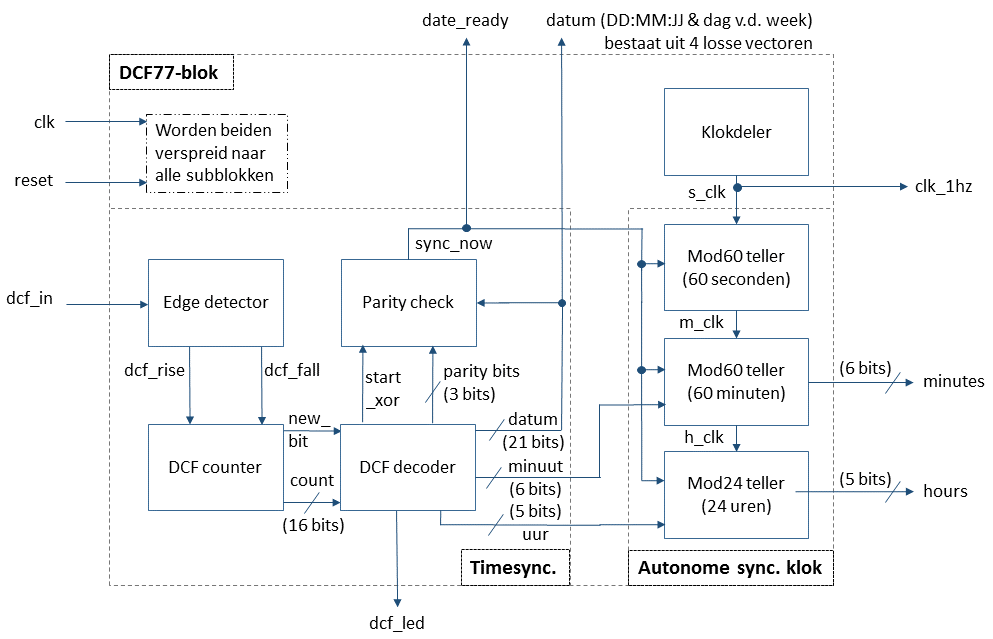
\includegraphics[keepaspectratio=true,scale=0.75]{Figuren/DCF77/Blokdiagram.png}
\caption{Verdeling van het DCF blok in subblokken}
\label{fig: dcf_subblokken}
\end{center}
\end{figure}

\subsection{FSM diagrammen}
Het opdelen van het grote DCF77 blok in subblokken is bijzonder nuttig, maar nog niet voldoende om direct een implementatie in VHDL te kunnen maken. Daarom wordt voor alle subblokken op het laagste abstractieniveau een FSM diagram gemaakt, waarin globaal wordt aangegeven wat er wanneer dient te gebeuren binnen elk van deze blokken. Er zijn in totaal acht verschillende subblokken te ontwerpen. Dit betekent dat er ook acht verschillende FSM diagrammen dienen te worden getekend. Bij wijze van voorbeeld wordt hier het FSM diagram van de parity\_check besproken. Alle acht FSM diagrammen zijn terug te vinden in \cref{Ap: dcf_fsm} als \cref{fig: edge_detector} t/m \cref{fig: uren_teller}.\\

\begin{figure}[h!]
\begin{center}
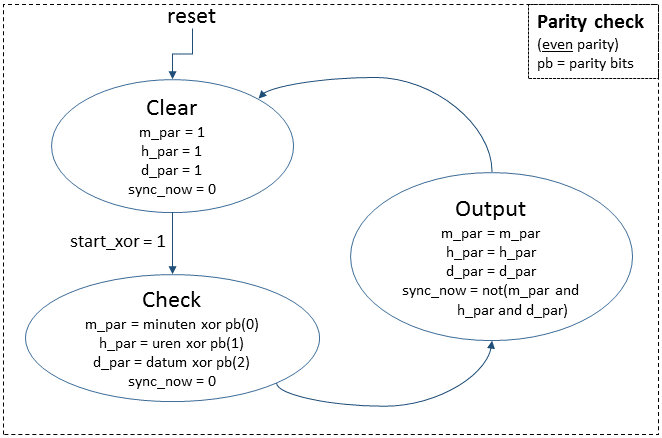
\includegraphics[keepaspectratio=true,scale=0.7]{Figuren/DCF77/FSM_parity_check}
\captionsetup{justification=centering}\caption{FSM diagram van het subblok parity check}
\label{fig: parity_check2}
\end{center}
\end{figure}

\noindent In \cref{fig: parity_check2} is het FSM diagram van de parity check nogmaals weergegeven. Zoals te zien is, begint deze na een reset altijd in de clear state. In tegenstelling tot wat je zou verwachten, worden in deze state de drie bits die het resultaat van de drie parity checks bevatten, niet op een logische 0, maar op een logische 1 gezet. Dit is zo, omdat in het DCF77 signaal gebruik wordt gemaakt van even parity. Dit betekent dat een parity bit een logische 0 bevat, wanneer de bijbehorende bitreeks een even aantal logische enen bevat. Een xor operatie met deze bitreeks + de bijbehorende parity bit zal dus 0 opleveren wanneer de parity bit correct is. In de reset ga je er echter juist vanuit dat de parity nog niet correct is. Wanneer dit door de decoder wordt aangegeven met het signaal start\_xor, zal de state van het subblok parity\_check naar check gaan.\\

\noindent In de state check worden vervolgens, door middel van herhaalde xor operaties, de daadwerkelijke parity checks uitgevoerd. \'E\'en check controleert de minuten, een tweede controleert de uren en de derde controleert de volledige datum (inclusief dag van de week). Onafhankelijk van het resultaat van deze drie parity checks, zal het subblok vervolgens gelijk naar de state output gaan.\\

\noindent In de state output worden dan de resultaten van de drie parity checks bij elkaar genomen. Dit gebeurt, om zo een strengere controle op de correctheid van de ontvangen bits te verkrijgen. Bovendien is op deze manier slechts \'e\'en signaal nodig dat aangeeft of de ontvangen tijd en datum correct zijn. Alleen als alle parity checks kloppen, zal het uitgangssignaal sync\_now hoog worden gemaakt. Hiermee worden vervolgens de tijd en datum vrijgegeven voor verder gebruik in de wekker. Ten slotte zal het subblok direct na het uitzenden van een puls op het sync\_now signaal weer teruggaan naar de state clear, zodat deze klaar staat om de volende minuut weer de parity checks uit te voeren. De cirkel is nu rond.

\subsection{VHDL code}
Met behulp van de FSM diagrammen kan er behavioural VHDL worden geschreven, welke vervolgens met behulp van structural VHDL aan elkaar kan worden gemaakt om zo uiteindelijk het hele DCF77 blok te vormen. Al deze behavioural en structural VHDL beschrijvingen zijn voorzien van enig commentaar en opgenomen in \cref{Ap: DCF_code}. Vanuit de top-level beschrijving in \cref{code: dcf77} is, eventueel met behulp van \cref{fig: dcf_subblokken}, gemakkelijk terug te vinden hoe alle andere VHDL beschrijvingen binnen het blok samenwerken.

\section{Simulatie}
Om de correcte functionaliteit te toetsen aan de verwachtingen, wordt de VHDL beschrijving van het DCF77 blok veelvuldig gesimuleerd. Hiervoor dienen echter wel testbenches geschreven te worden, welke het te testen onderdeel voorzien van testsignalen. Deze testbenches zijn voor ieder apart onderdeel geschreven in twee varianten, ook voor de structural beschrijvingen. In de eerste variant wordt er vanuit gegaan dat de systeemklok, net als in het uiteindelijke product, een signaal van 32 kHz is. Op deze variant van de testbenches wordt in dit verslag verder niet ingegaan, omdat deze te lang zijn. Dit levert later in het proces problemen op tijdens het simuleren op transistorniveau. Daarom is er ook een tweede variant van alle testbenches geschreven, waarin gebruik wordt gemaakt van geschaalde ingangssignalen. Op deze manier is er een veel kortere simulatietijd nodig, terwijl toch uit de resultaten opgemaakt kan worden of het geteste onderdeel naar verwachting werkt. Deze testbenches zijn opgenomen in \cref{Ap: DCF_test} als \cref{code: edge_detector_tb} t/m \cref{code: dcf77_tb}\\

\noindent In \emph{Modelsim} worden vervolgens alle onderdelen van het DCF77 blok getest op behavioural niveau met behulp van deze testbenches. Zodra de resultaten van deze simulaties overeenkomen met de verwachte resultaten, worden alle VHDL beschrijvingen in het programma \emph{GoWithTheFlow} gesynthetiseerd. De gesynthetiseerde VHDL kan vervolgens met dezelfde testbenches opnieuw in \emph{Modelsim} worden gesimuleerd. Als alles goed is, zullen de resultaten er precies hetzelfde uitzien. In dat geval wordt er van alle subblokken een layout gegenereerd door de programma's \emph{Madonna} \& \emph{Trout}. Uit deze layout kan vervolgens binnen \emph{GoWithTheFlow} weer VHDL worden ge\"extraheerd. Deze VHDL kan vervolgens opnieuw met dezelfde testbenches in \emph{Modelsim} worden gestopt ter controle. Ook de resultaten van deze simulaties zullen als alles klopt precies hetzelfde zijn als die van de behavioural simulaties. Binnen \emph{GoWithTheFlow} is het echter ook mogelijk om aan de hand van een testbench de gegenereerde layout direct, zonder extractie van VHDL, te simuleren. Dit heet ook wel de switch-level simulatie, omdat deze het ontwerp op transistorniveau simuleert. Ten slotte is het binnen \emph{GoWithTheFlow} mogelijk om de resultaten van de switch-level simulatie te laten vergelijken met die van de behavioural simulatie. Als ze met elkaar overeen komen, mag deze vergelijking slechts \'e\'en enkele error opleveren; namelijk direct aan het begin van de simulatie, wanneer er nog ge\"initialiseerd wordt.

\section{Rapid prototyping (FPGA implementatie)}

\section{Resultaten}